\section{Modelul informaţional pentru microunde - ONF TR-532 (\textit{Microwave Information Model})}

Modelul informațional pentru microunde \cite{onftr532} a apărut in Decembrie 2016 ca o recomandare formulată de grupul \gls{otwg} din cadrul \gls{onf}. Scopul acestuia este de a modela un echipament de transport de date fără fir, pentru a putea fi folosit de echipamentele de control \gls{sdn}, în încercarea de a asigura o independenţă față de producătorii de echipamente. Chiar dacă este denumit \textit{model informațional pentru microunde}, acesta poate fi aplicat fără probleme nu numai echipamentelor ce funcționează în spectrul microundelor, ci și echipamentelor care funcționează în benzi de frecvenţă mai înalte (lungimi de undă milimetrice), care încep să își facă tot mai mult simţită prezenţa în rețelele actuale de transport.

\begin{figure}[t]
	\centering
	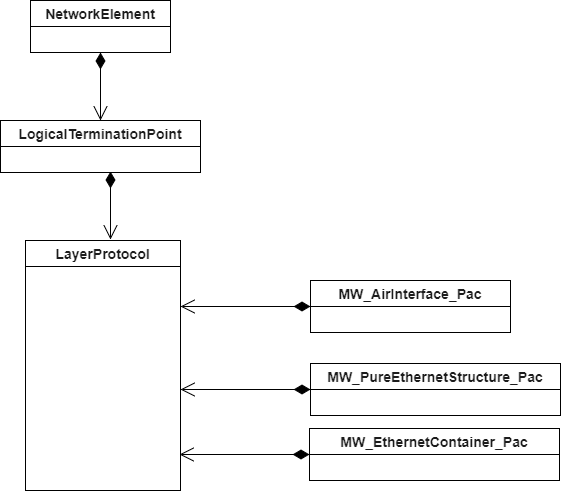
\includegraphics[width=1\textwidth]{microwave_model_overview}
	\caption{Reprezentare UML simplificată a \textit{MicrowaveModel}}
	\label{fig:microwave_model}
\end{figure}


TR-532 este de fapt o extensie specifică tehnologiei \gls{wt} a modelului informațional de bază, versiunea 1.2 (TR-512.1). Astfel, conţine mai multe pachete condiţionale caracteristice acestei tehnologii. O vedere de ansamblu simplificată a acestui model, împreună cu legătura acestuia cu \textit{CoreModel} este ilustrată în Figura \ref{fig:microwave_model}.

În următoarele paragrafe se vor detalia obiectele acestui model care sunt importante din punctul de vedere al simulatoarelor dezvoltate în această lucrare.

\subsection{Obiectul \textit{MW\_AirInterface\_Pac}}

\subsection{Obiectul \textit{MW\_PureEthernetStructure\_Pac}}

\subsection{Obiectul \textit{MW\_EthernetContainer\_Pac}}